\documentclass[dvipsnames]{beamer} % [draft/handout] (Schnellübersicht goo.gl/AS72B)
\mode<presentation>{
    \useoutertheme{infolines}
    \usecolortheme{dolphin} % Farbthema ab Besten selbst machen
    \usecolortheme{orchid}
}
\usepackage[T1]{fontenc} % Umlaute
\usepackage[utf8]{inputenc} % Textcodierung
\usepackage[ngerman]{babel} % Silbentrennung
\usepackage{marvosym, amsmath, amssymb} % Symbole, Formeln, amssymb > mathdesign
\usepackage{lmodern, microtype} % enhanced CM, mikrotypografische Feinheiten
\usepackage{xcolor}
\usepackage{hyperref}
\hypersetup{
	colorlinks = true,
	allcolors = ,
	urlcolor = blue!75
}
\usepackage{booktabs, tabularx}
\usepackage{listings}
\lstset{
	basicstyle=\ttfamily,
	columns=flexible,
	breaklines=true,
	numbers=left,
	%xleftmargin=0.5cm,
	tabsize=4,
	numberstyle=\scriptsize\color{gray},
	stringstyle=\color{orange},
	commentstyle=\color{teal},
	keywordstyle=\bfseries\color{Blue},
	backgroundcolor=\color{black!05},
	% Special
	breakindent=0cm,
  moredelim=[is][\bfseries\color{Red}]{@}{@},
}

%\includeonlyframes{current} % FIXME

\providecommand{\attribution}[4]{\textcolor{gray}{\tiny \href{#1}{Illustration} by #2 / \href{#3}{#4}}}
\DeclareMathOperator*{\argmax}{arg\,max} % FIXME

\title[BitTorrent-Downloads]{Analysis of BitTorrent Trackers and Peers}
\subtitle{Counting Confirmed Downloads in BitTorrent}
\author{Stefan Schindler}
\institute[FAU]{Friedrich-Alexander-Universität Erlangen-Nürnberg}
\date{13. Oktober 2015}
\subject{Bachelor Thesis}

\AtBeginSection[]{
    \begin{frame}<beamer>{Agenda}
        \tableofcontents[currentsection]
    \end{frame}
}

\begin{document}
	\shorthandoff{"}
	\begin{frame}
		\titlepage
	\end{frame}

%%%%%%%%%%%%%%%%%%%%%%%%%%%%%%%%%%%%%%%%%%%%%%%%%%%%%%%%%%%%%%%%%%%%%%%%%%%%%%%%%%
	\begin{frame}{Agenda}
		\tableofcontents
	\end{frame}

%%%%%%%%%%%%%%%%%%%%%%%%%%%%%%%%%%%%%%%%%%%%%%%%%%%%%%%%%%%%%%%%%%%%%%%%%%%%%%%%%%
	\section{Einleitung, Motivation und Aufgabe}
	\begin{frame}{Einleitung, Motivation und Aufgabe}
		% TODO BEPs
	\end{frame}

%%%%%%%%%%%%%%%%%%%%%%%%%%%%%%%%%%%%%%%%%%%%%%%%%%%%%%%%%%%%%%%%%%%%%%%%%%%%%%%%%%
	\section{Funktionsweise von BitTorrent}
	\subsection{BitTorrent-Protokoll}
	\begin{frame}{Funktionsweise von BitTorrent}
		\begin{columns}
			\column{0.5\textwidth}
			\begin{itemize}
				\item Datei oder Verzeichnis
				\item Einteilung in Segmente
				\item Peer-to-Peer-Datenübertragung
				\item Übergang von Leecher zu Seeder
				\item Integritätsprüfung mit SHA-1
			\end{itemize}
			\column{0.5\textwidth}
			\centering
	    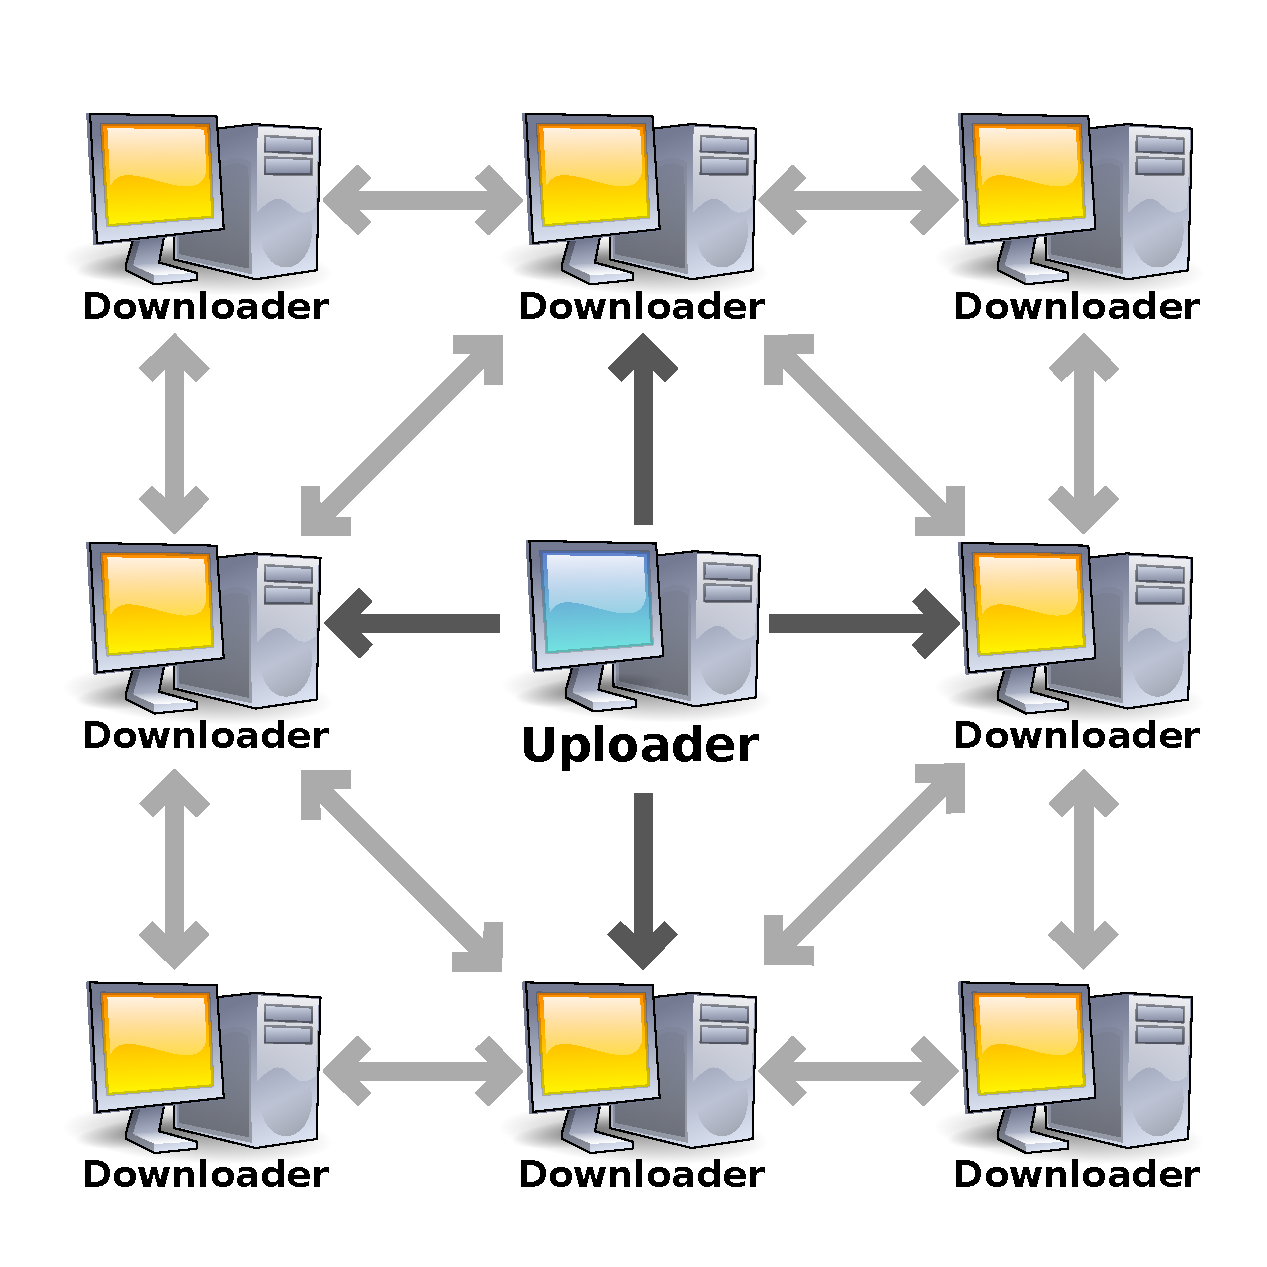
\includegraphics[width=\textwidth]{001_BitTorrent_network}\\
	    \attribution{https://commons.wikimedia.org/wiki/File:BitTorrent_network.svg}{Scott Martin}{https://creativecommons.org/licenses/by-sa/3.0/deed.en}{CC SA}
		\end{columns}
	\end{frame}

	\begin{frame}[fragile]{Bencoding und Torrent-Datei}
		\begin{center}
			\begin{tabular}{lll}
				\toprule
				Datentyp & Bencoding & Beispiel \\
				\midrule
				String & \texttt{<length>:<string>} & \texttt{3:aaa} = \texttt{"aaa"} \\
				Integer & \texttt{i<integer>e} & \texttt{i23e} = \texttt{23} \\
				List & \texttt{l<val1>...e} & \texttt{l3:aaai23ee} = \texttt{["aaa", 23]} \\
				Dictionary & \texttt{d<key1><val1>...e} & \texttt{d3:aaai23ee} = \texttt{\{"aaa": 23\}} \\
				\bottomrule
			\end{tabular}
		\end{center}

		\pause
		\begin{itemize}
			\item Metainfo-Datei mit \texttt{.torrent} Dateisuffix
			\begin{lstlisting}
d@8:announce@41:http://bttracker.debian.org:6969/announce@4:info@d@4:name@28:debian-8.0.0-amd64-DVD-1.iso@6:length@i3976200192e@12:piece length@i1048576e@6:pieces@75840:<hashes>ee
			\end{lstlisting}
		\end{itemize}
	\end{frame}

	\begin{frame}[fragile]{Peeranfrage an Tracker-Server}
		\begin{itemize}
			\item Peer-Adressen anfordern und Teilnahme bekanntgeben
				\begin{lstlisting}
	http://bttracker.debian.org:6969/@announce@?@info_hash@=W%E1Y%A5%82a%C8%D2%F4%2Ad%98%0D%2B%80%8E9%01%FC%F6&@port@=6881&@peer_id@=hNsfr5PYlFtWO73yvSGX&@event@=started&@downloaded@=1896&@left@=1896&@uploaded@=758
				\end{lstlisting}
			\pause
			\item Statistikabfrage über Leecher, Seeder, abgeschlossene Downloads
				\begin{lstlisting}
	http://bttracker.debian.org:6969/@scrape@?@info_hash@=W%E1Y%A5%82a%C8%D2%F4%2Ad%98%0D%2B%80%8E9%01%FC%F6
				\end{lstlisting}
			\pause
			\item UDP-basiertes Protokoll als effizientere Alternative
		\end{itemize}
	\end{frame}

	\begin{frame}{Nachrichten im Peer-Protokoll}
		\begin{description}[(un-)\,choke, (not) interested]
			\item[handshake] Protokollversion, Infohash, Erweiterungen
			\item[(un-)\,choke, (not) interested] Bandbreitenverwaltung
			\item[\alert{bitfield, have}] Angebot an Segmenten
			\item[request, cancel] Anforderung von Segmenten
			\item[piece] Nutzdaten
			\item[port] DHT-Port
		\end{description}
	\end{frame}

	\subsection{DHT-Netzwerk}
	\begin{frame}{Peeranfrage im DHT-Netzwerk}
		\begin{itemize}
			\item DHT-Knoten in jedem Client mit eigener ID
			\begin{itemize}
				\item \alert{Routingtabelle} mit Nachbar-Knoten
				\item \alert{Infohash-Tabelle} mit Peeradressen
			\end{itemize}
			\item Knoten nahe dem Infohash \alert{iterativ} finden
			\item Nahe Knoten liefern Peeradressen
			\item Torrent-Teilnahme anderen Knoten mitteilen
		\end{itemize} % FIXME Magnet-Link aufschreiben oder erwähnen

		\begin{center}
			1 \\
			2 \\
			3 \\
			(Illustration Lookup siehe Tafel) \\ % TODO
			5 \\
			6 \\
			7
		\end{center}
	\end{frame}

%%%%%%%%%%%%%%%%%%%%%%%%%%%%%%%%%%%%%%%%%%%%%%%%%%%%%%%%%%%%%%%%%%%%%%%%%%%%%%%%%%
	\section{BitTorrent Download Analyzer}
% 	\begin{frame}{Abhängigkeiten} % FIXME
% 	\end{frame}

	\subsection{Arbeitsweise}
	\begin{frame}{Arbeitsweise des Analysewerkzeugs}
		\begin{enumerate}
			\item \alert{Import} von Torrent-Dateien und Magnet-Links
			\item \alert{Adressen} in Peer-Warteschlange sammeln
			\begin{itemize}
				\item Von Tracker-Server
				\item Aus DHT-Netzwerk
			\end{itemize}
			\item \alert{Download-Fortschritt} in DB-Warteschlange schreiben
			\begin{itemize}
				\item Peers aktiv kontaktieren
				\item Passiv Verbindungen annehmen
			\end{itemize}
			\item Peers in \alert{Datenbank} aktualisieren, zurücklegen in Peer-Warteschlange
		\end{enumerate}

		\vspace{0.5cm}
    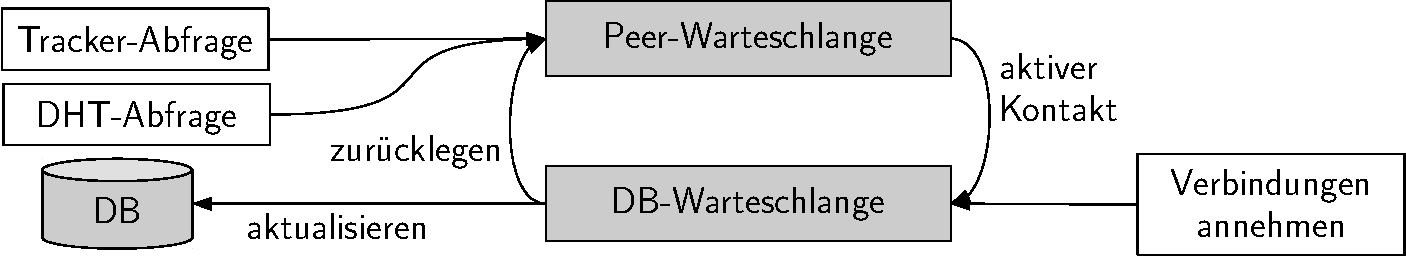
\includegraphics[width=\textwidth]{002_Komponenten-crop}
	\end{frame}

% 	\begin{frame}{Wichtige Parameter} % FIXME
% 	\end{frame}

	\subsection{Einschränkungen}
	\begin{frame}{Einschränkungen des Analysewerkzeugs}
		Nicht unterstützte Technologien:

		\begin{itemize}
			\item IPv6 bei Tracker-Abfragen und DHT-Netzwerk
			\item uTP (Micro Transport Protocol)
			\item PEX (Peer Exchange)
			\item TEX (Tracker Exchange)
			\item Azureus-DHT-Netzwerk
		\end{itemize}
	\end{frame}

%%%%%%%%%%%%%%%%%%%%%%%%%%%%%%%%%%%%%%%%%%%%%%%%%%%%%%%%%%%%%%%%%%%%%%%%%%%%%%%%%%
	\section{Auswertung}
	\begin{frame}{Auswahl von Torrents}
	\end{frame}

	\begin{frame}{Adresssammlung}
	\end{frame}

	\begin{frame}{Bestätigte Downloads}
	\end{frame}

	\begin{frame}{Methodische Probleme}
	\end{frame}

	\subsection{Geographische Analyse}
	\begin{frame}{Häufigkeit der Herkunftsländer}
    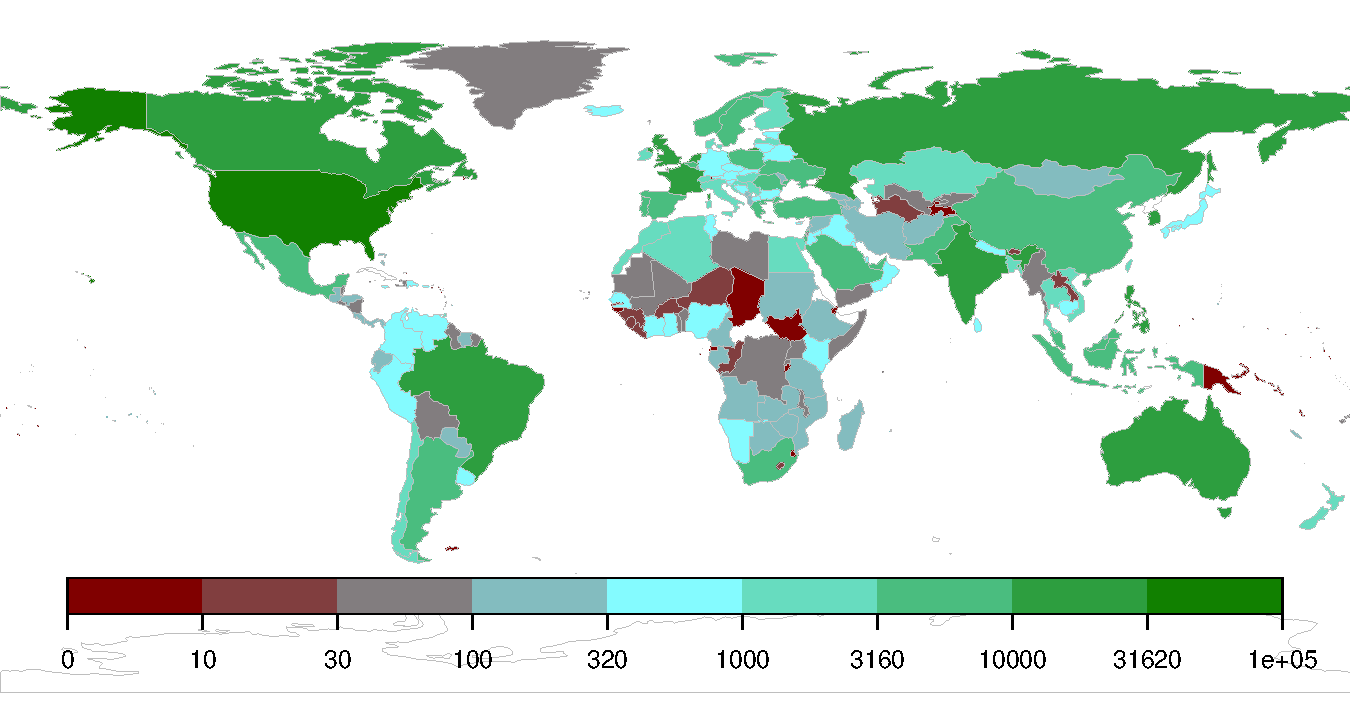
\includegraphics[width=\textwidth]{2015-08-30_20-combined_location_map}
	\end{frame}

	\begin{frame}{Mittlere Download-Geschwindigkeiten}
    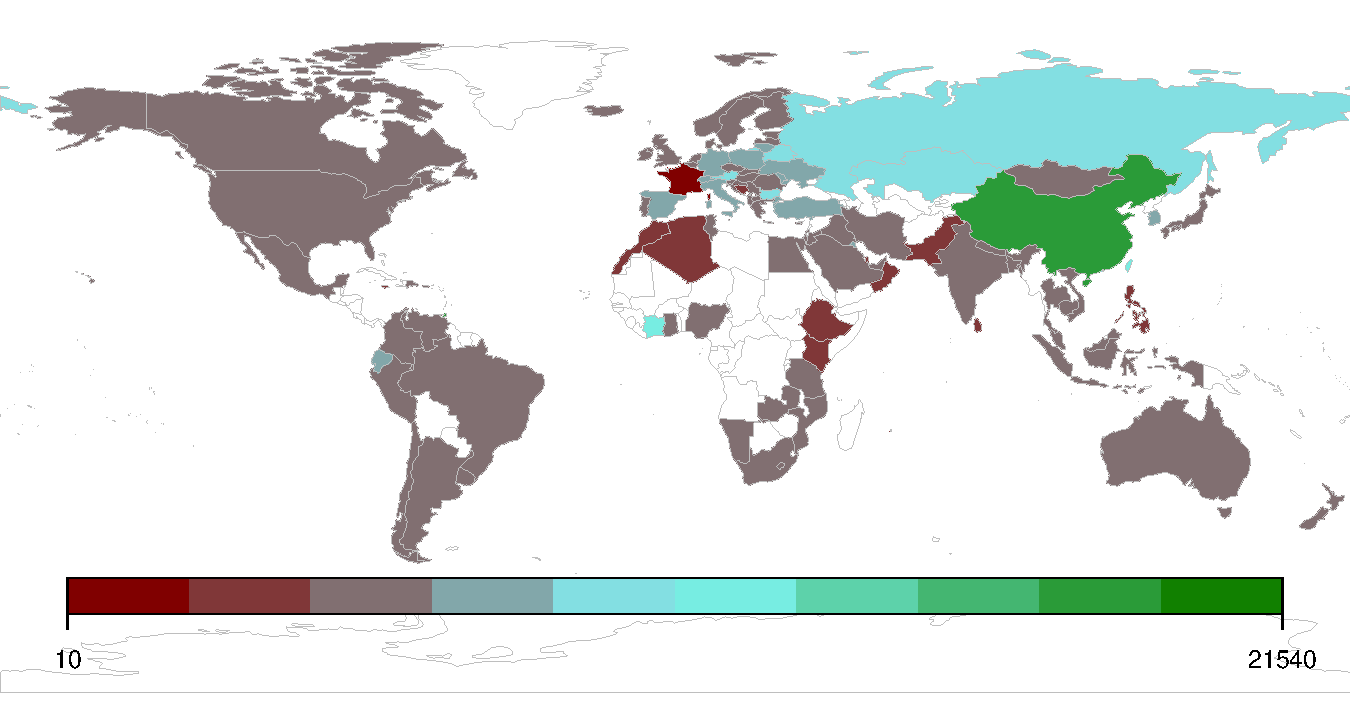
\includegraphics[width=\textwidth]{2015-08-30_20-combined_speed_map}
	\end{frame}

%%%%%%%%%%%%%%%%%%%%%%%%%%%%%%%%%%%%%%%%%%%%%%%%%%%%%%%%%%%%%%%%%%%%%%%%%%%%%%%%%%
	\section{Fazit und Ausblick}
	\begin{frame}{Fazit und Ausblick}
	\end{frame}

%%%%%%%%%%%%%%%%%%%%%%%%%%%%%%%%%%%%%%%%%%%%%%%%%%%%%%%%%%%%%%%%%%%%%%%%%%%%%%%%%%
	\begin{frame}{Zusammenfassung}
		% TODO oder eigene Sätze
		\tableofcontents
	\end{frame}
\end{document}
